\documentclass[a4paper,12pt]{report}

\usepackage{alltt, fancyvrb, url}
\usepackage{graphicx}
\usepackage[utf8]{inputenc}
\usepackage{float}
\usepackage{hyperref}


\title{OOP Java project \\Budmate:\\ Personal budget manager}

\author{
    alessandro.stefani10@studio.unibo.it \\
    giulio.salotti@studio.unibo.it \\
    paolo.pietrelli@studio.unibo.it \\
    zhaohui.song@studio.unibo.it
}

\date{\today}

\begin{document}

\maketitle

\tableofcontents

\chapter{Analisi}

\section{Requisiti}

In the year 2022 due to the federal reserve's decision, a lot of liquidity floods into the market, many people are lured in to make some bucks.
But the market is like an ocean, teeming with volatilities. 
Though various platforms have emerged, we lacked a tool to manage every income and expenditure, our idea is to build a cloud-based platform that connects to various markets, provides analysis tools to clients to minimize the risk, and get the big picture of actual assets. .
It's a tiny project of about 80 hours amount of work, hence it will only be a prototype.

\subsection*{Elementi positivi}
\begin{itemize}
	\item The software should be able to manage various assets of a client.
	\item management of one or more profiles including registration and switching between accounts.
	\item account management, piggy banks, investment management, and expense management.
	\item vision of the stock and crypto markets.
\end{itemize}

\subsection*{Elementi negativi}
\begin{itemize}
	\item This software depends on if a platform such as \textit{Binance} \footnote{\url{https://www.binance.com/en/binance-api}} gives an open API, then your action on the budmate will actually be executed on the Binance platform.
\end{itemize}

\subsection*{Esempio}
This software was supposed to provide visual tools to analyze market conditions, but it will be implemented once all basic functionalities are satisfied.
%
Such as using deep learning to analyze future accounts' conditions based on the historic data. (Backtracking).

\subsubsection{Requisiti funzionali}
\begin{itemize}
	\item There should be a login and registration screen upon software's activation, authentication of profile via database or google / Facebook authenticator.
    \item A profile page contains everything about the user, including total value, number of accounts, activities, subscription plan, whether the client needs to pay fees or not, and even accessing friends' pages.
    \item Investment page: an overview of all assets owned on various platforms, a chart showing the trend of the total value of the investments. The ability to purchase and sell assets, such as BITCOIN, and APPLE. In the future, there will also be NFT markets, government bonds, real estate, and maybe even gaming assets(metaverse).
    \item Accounts page: Bank accounts, investment accounts, Budmate accounts, with various information containing IBAN, and swift code. 
    The ability to create or connect to an existing bank account, whether is Uni credit or Goldman Sachs.
    \item Expenditure page:  shows various kinds of expenses done in the shopping mall, grocery store, book shop, restaurants, cafe bar, monthly subscriptions, student loans, and charts with visual future trends.
\end{itemize}

\subsubsection{Requisiti non funzionali}
\begin{itemize}
    \item For the workflow, we use git and develop the software on different machines and OS, including windows, ubuntu 22.04, 20.04, and macOS. 
    \item The architecture of software should be highly independent, If one member couldn't work full time, that shouldn't bother the others' work.
\end{itemize}

\section{Analisi e modello del dominio}
Our app starts from the profile class, in the profile, there can be many types of accounts: 
such as expenses, bank accounts, investment accounts, holding accounts, and even Budmate accounts. Those accounts have similar functionalities, in below, you can find specific implementations.

\subsection*{Elementi positivi}
\begin{itemize}
	\item easy structure, simple responsibility.
	\item independent implementation without depending on the other's realization, the use of interface.
\end{itemize}

\subsection*{Elementi negativi}
\begin{itemize}
	\item Its functionality is dependent on access to the internet, If a user is offline, it's hard to do any trading operation.
\end{itemize}

\subsection*{Esempio}
You can see the architecture below.

\begin{figure}[H]
\centering{}
\makebox[\textwidth][c]{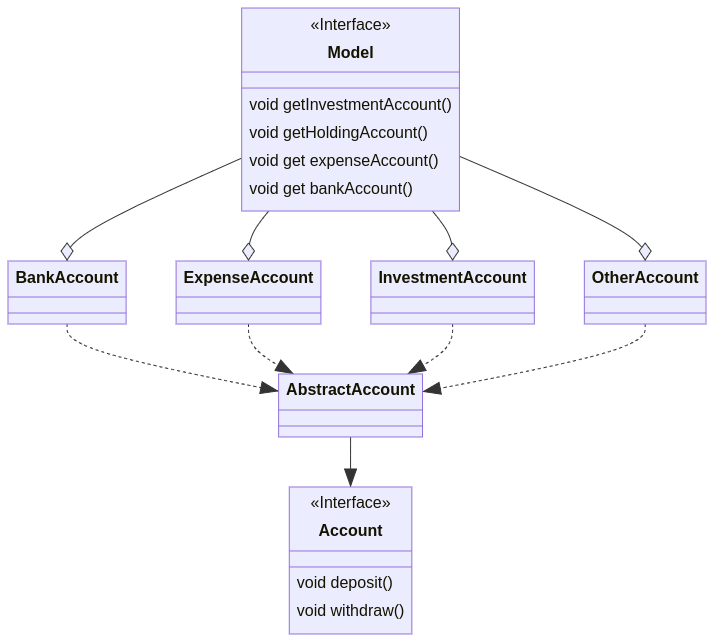
\includegraphics[width=1.2\textwidth]{img/domainAnalysis.png}}%
\caption{Our structure of model}
\label{img:domainAnalysis}
\end{figure}

\chapter{Design}
Our design fulfills tremendously \textit{5 design principles}
\subsection*{principles}
\begin{itemize}
	\item DRY: Don’t repeat yourself 
    \item KISS: Keep it simple, stupid 
    \item SRP: Single Responsibility Principle
    \item OCP: Open-clodes principle
    \item DIP: Dependency-inversion principle
\end{itemize}

\section{Architettura}
	We use design pattern MVC(view, control, model) for our whole structure, we use JavaFX for our view and other views for logging.  
	A controller that gets notified by JavaFX event, access model for computation then updates the view.  

\subsection*{Elementi positivi}
\begin{itemize}
	\item By using MVC and Interface, we can switch between JavaFX and other graphic libraries without changing other parts. 
    \item We use other threads to compute tasks that uses a lot of time.
\end{itemize}

\subsection*{Elementi negativi}
\begin{itemize}
	\item We asked many people and in the forum, but it seems we couldn't create a reference of the controller without being static.
\end{itemize}

\subsection*{Esempio}

Even though using the private static volatile controller is a bad solution, it works correctly with synchronization between the thread from the controller and the components on the JavaFX thread. 
I have been working on that for more than 15 hours, but still couldn't find a solution. In this case, we have multiple views, each of them is attached to the one controller, it wasn't something that we didn't intend to do.
Instead on the he part of controller, all views are accessible from a thread pool created by Executor services. 

\begin{figure}[H]
	\centering{}
	\makebox[\textwidth][c]{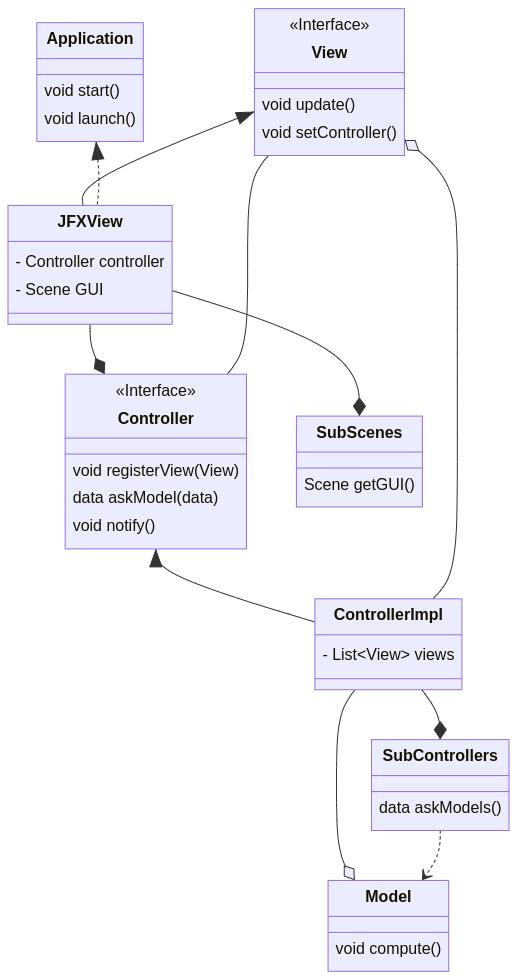
\includegraphics[width=0.75\textwidth]{img/MVC.png}}%
	\caption{Our structure of MVC implementation}
	\label{img:MVC}
	\end{figure}

%%\Cref{img:} è esemplificato il diagramma UML architetturale.


\section{Design dettagliato}

\subsection*{Zhaohui Song}

Since I started the project earlier than the others, I feel that I don't want the others to rewrite the same piece of code multiple times, so every design should at least satisfy DRY OCP, either for the Model or the GUI.
%
\\\\Some patterns are perfectly fit for my solution including the \textit{Factory method, Builder, Template method, Iterator, Strategy, Observer, and Decorato}r, I avoided \textit{singleton} as much as possible.
%
\\\\Some functions are left open because as mentioned above, we may need to add the third-party API to fulfill the order done by the client. Like if a user Bob wants to buy a share of Amazon stock since our app is a kind of portfolio tracker,  
he can hit the button Buy in our app, then our app will send the order to the actual broker app, the advantage is you can analyze the data using our app, then executing the order automatically to various platform, in the case one platform bankrupts, you won't lose everything.
%
\\\\You may not see all implementations of these functionalities, but I think when it comes to design an app, I ought to make it equipped with  \textbf{scalability,  interoperability}(coherent with other existing apps, because I don't want to write something that already exists), \textbf{standardized, feature-complete, and easy for the rest of team members to develop}.
And by thinking that, I used most of my 80 hours to make it easier for the others use.
%
\subsubsection*{Generalise Account as much as possible and create my part InvestmentAccount}
\begin{figure}[H]
	\centering{}
	\makebox[\textwidth][c]{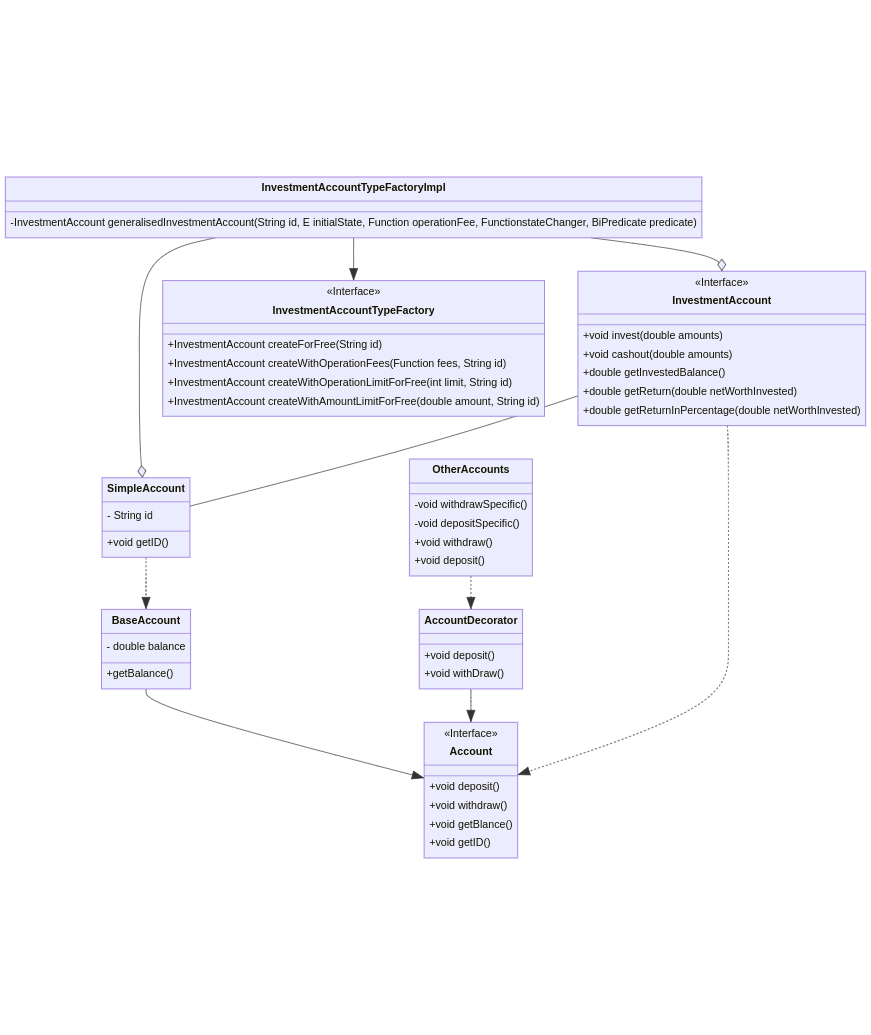
\includegraphics[width=1.7\textwidth]{img/invAccount.png}}%
	\caption{generalised Account}
	\label{img:invAccount}
	\end{figure}

	\paragraph{Problem:} Make an account interface that's common to everybody

	\paragraph{Solution:} An interface that satisfies basic operations such as deposit and withdrawal. In my opinion, all accounts are basically simple accounts, So you can either extend it to make a more detailed realization or implement \textbf{\textit{decorators}} to add single responsibilities to the easy account, or even use it as a component as I did in my investment account factory.

	\paragraph*{Problem:} When this app is ready, I need to think about how to make a profit, depends on the current user's description plan, we may charge a fee to his trading operation, add a limit to the number of times, and add the limit amount for withdrawal, etc. 

	\paragraph*{Solution:} As I will have multiple genres of investment Accounts, I create a factory that builds different investment accounts for me. Here I used \textbf{strategy}(function and bipredicate) via lambda expression for how to charge a fee form client;
	An initial state with a generic type to define based on what factor a limit can be added. The pattern used here consists of the \textbf{Factory method, template method}. 


\subsubsection*{Need a place to trade stocks with the real-time price change}
	\begin{figure}[H]
	\centering{}
	\makebox[\textwidth][c]{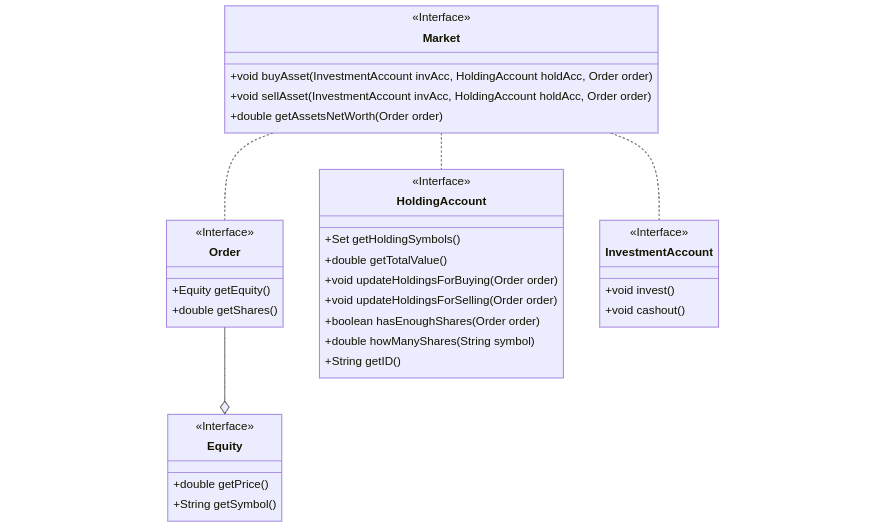
\includegraphics[width=1.3\textwidth]{img/market.png}}%
	\caption{market}
	\label{img:market}
	\end{figure}

	\paragraph{Problem:} How to trade generalised assets with real-time prices

	\paragraph*{Solution:} Here I generalize every kind of asset into class Equity, which can be either stock, cryptos, NFTs, commodities, ETFs, etc. All we need is a symbol and its price. As you see in the figure above, when a user trade with a symbol, assets will be added to the holding account, and money will be decreased in the corresponding investment account.

\subsubsection*{A group of database to retrieve real world information}
\begin{figure}[H]
	\centering{}
	\makebox[\textwidth][c]{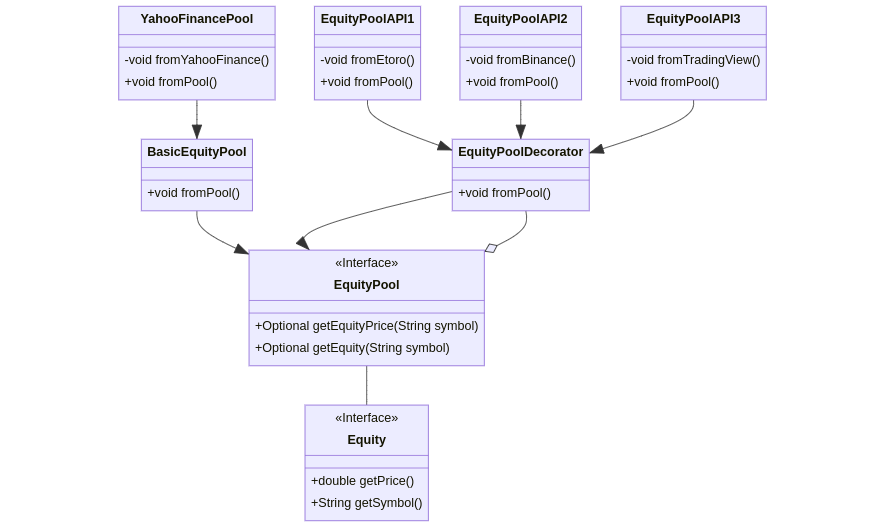
\includegraphics[width=1.3\textwidth]{img/EquityPool.png}}%
	\caption{EquityPool}
	\label{img:EquityPool}
	\end{figure}

	\paragraph{Problem:} How to query prices from more platforms

	\paragraph*{Solution:}Using the design pattern \textbf{decorator} perfectly resolved this problem, firstly we search the price on our default platform Yahoo Finance. In the case we know that an asset may not be found there, we can add more layers for searching from other platforms. It's like a cache hit(how the CPU uses cache to find data in the memory). If the price can be found in the cache of level 1, then that's it, otherwise, it will searches from the cache level 2...n till the central memory. 
	As an example, if a user were searching for a 10-year government bond, it's likely that it won't appear in the market. Then we can do Equity eq = new EquityPoolApiBond(new YahooFinancePool());  So we cover the searching as much as possible.


\chapter{Sviluppo}
\section{Testing automatizzato}

Il testing automatizzato è un requisito di qualunque progetto software che si rispetti, e consente di verificare che non vi siano regressioni nelle funzionalità a fronte di aggiornamenti.
%
Per quanto riguarda questo progetto è considerato sufficiente un test minimale, a patto che sia completamente automatico.
%
Test che richiedono l'intervento da parte dell'utente sono considerati \textit{negativamente} nel computo del punteggio finale.

\subsection*{Elementi positivi}

\begin{itemize}
 \item Si descrivono molto brevemente i componenti che si è deciso di sottoporre a test automatizzato.
 \item Si utilizzano suite specifiche (e.g. JUnit) per il testing automatico.
 \item Se sono stati eseguiti test manuali di rilievo, si elencano descrivendo brevemente la ragione per cui non sono stati automatizzati. Ad esempio, se tutto il team sviluppa e testa su uno stesso sistema operativo e si sono svolti test manuali per verificare, ad esempio, il corretto funzionamento dell'interfaccia grafica o di librerie native su altri sistemi operativi, può avere senso menzionare la cosa.
\end{itemize}

\subsection*{Elementi negativi}
\begin{itemize}
 \item Non si realizza alcun test automatico.
 \item La non presenza di testing viene aggravata dall'adduzione di motivazioni non valide. Ad esempio, si scrive che l'interfaccia grafica non è testata automaticamente perché è \emph{impossibile} farlo\footnote{Testare in modo automatico le interfacce grafiche è possibile (si veda, come esempio, \url{https://github.com/TestFX/TestFX}), semplicemente nel corso non c'è modo e tempo di introdurvi questo livello di complessità. Il fatto che non vi sia stato insegnato come farlo non implica che sia impossibile!}.
 \item Si descrive un testing di tipo manuale in maniera prolissa.
 \item Si descrivono test effettuati manualmente che sarebbero potuti essere automatizzati, ad esempio scrivendo che si è usata l'applicazione manualmente.
 \item Si descrivono test non presenti nei sorgenti del progetto.
 \item I test, quando eseguiti, falliscono.
\end{itemize}

\section{Metodologia di lavoro}

Ci aspettiamo, leggendo questa sezione, di trovare conferma alla divisione operata nella sezione del design di dettaglio, e di capire come è stato svolto il lavoro di integrazione.
%
\textbf{Andrà realizzata una sotto-sezione separata per ciascuno studente} che identifichi le porzioni di progetto sviluppate, separando quelle svolte in autonomia da quelle sviluppate in collaborazione.
%
Diversamente dalla sezione di design, in questa è consentito elencare package/classi, se lo studente ritiene sia il modo più efficace di convogliare l'informazione.
%
Si ricorda che l'impegno deve giustificare circa 40-50 ore di sviluppo (è normale e fisiologico che approssimativamente la metà del tempo sia impiegata in analisi e progettazione).

\subsection*{Elementi positivi}

\begin{itemize}
	\item Si identifica con precisione il ruolo di ciascuno all'interno del gruppo, ossia su quale parte del progetto ciascuno dei componenti si è concentrato maggiormente.
	\item La divisione dei compiti è equa, ossia non vi sono membri del gruppo che hanno svolto molto più lavoro di altri.
	\item La divisione dei compiti è coerente con quanto descritto nelle parti precedenti della relazione.
	\item La divisione dei compiti è realistica, ossia le dipendenze fra le parti sviluppate sono minime.
	\item Si identifica quale parte del software è stato sviluppato da tutti i componenti insieme.
	\item Si spiega in che modo si sono integrate le parti di codice sviluppate separatamente, evidenziando eventuali problemi. Ad esempio, una strategia è convenire sulle interfacce da usare (ossia, occuparsi insieme di stabilire l'architettura) e quindi procedere indipendentemente allo sviluppo di parti differenti. Una possibile problematica potrebbe essere una dimenticanza in fase di design architetturale che ha costretto ad un cambio e a modifiche in fase di integrazione. Una situazione simile è la norma nell'ingegneria di un sistema software non banale, ed il processo di progettazione top-down con raffinamento successivo è il così detto processo ``a spirale''.
	\item Si descrive in che modo è stato impiegato il DVCS.
\end{itemize}

\subsection*{Elementi negativi}
\begin{itemize}
	\item Non si chiarisce chi ha fatto cosa.
	\item C'è discrepanza fra questa sezione e le sezioni che descrivono il design dettagliato.
	\item Tutto il progetto è stato svolto lavorando insieme invece che assegnando una parte a ciascuno.
	\item Non viene descritta la metodologia di integrazione delle parti sviluppate indipendentemente.
	\item Uso superficiale del DVCS.
\end{itemize}

\section{Note di sviluppo}

Questa sezione, come quella riguardante il design dettagliato va svolta \textbf{singolarmente da ogni membro del gruppo}.

Ciascuno dovrà mettere in evidenza eventuali particolarità del suo metodo di sviluppo, ed in particolare:
\begin{itemize}
	\item \textbf{Elencare} (fare un semplice elenco per punti, non un testo!) le feature \textit{avanzate} del linguaggio e dell'ecosistema Java che sono state
utilizzate. Le feature di interesse sono:
	\begin{itemize}
		\item Progettazione con generici, ad esempio costruzione di nuovi tipi generici, e uso di generici bounded. Uso di classi generiche di libreria non è considerato avanzato.
		\item Uso di lambda expressions
		\item Uso di \texttt{Stream}, di \texttt{Optional} o di altri costrutti funzionali
		\item Uso della reflection
		\item Definizione ed uso di nuove annotazioni
		\item Uso del Java Platform Module System
		\item Uso di parti di libreria non spiegate a lezione (networking, compressione, parsing XML, eccetera...)
		\item Uso di librerie di terze parti (incluso JavaFX): Google Guava, Apache Commons...
		\item Uso di build systems
	\end{itemize}
	Si faccia molta attenzione a non scrivere banalità, elencando qui features di tipo ``core'', come le eccezioni, le enumerazioni, o le inner class: nessuna di queste è considerata avanzata.
	\item Descrivere \textit{molto brevemente} le librerie utilizzate nella propria parte di progetto, se non trattate a lezione (ossia, se librerie di terze parti e/o se componenti del JDK non visti, come le socket). Si ricorda che l'utilizzo di librerie è valutato \emph{positivamente}.
	\item Sviluppo di algoritmi particolarmente interessanti \emph{non forniti da alcuna libreria} (spesso può convenirvi chiedere sul forum se ci sia una libreria per fare una certa cosa, prima di gettarvi a capofitto per scriverla voi stessi).
\end{itemize}
%
In questa sezione, \textit{dopo l'elenco}, è anche bene evidenziare eventuali pezzi di codice ``riadattati'' (o scopiazzati...) da Internet o da altri progetti, pratica che tolleriamo ma che non raccomandiamo.
%
I pattern di design, invece \textbf{non} vanno messi qui.
%
L'uso di pattern di design (come suggerisce il nome) è un aspetto avanzato di design, non di implementazione,
e non va in questa sezione.

\subsection*{Elementi positivi}

\begin{itemize}
	\item Si elencano gli aspetti avanzati di linguaggio che sono stati impiegati
	\item Si elencano le librerie che sono state utilizzate
	\item Si descrivono aspetti particolarmente complicati o rilevanti relativi all'implementazione,
ad esempio, in un'applicazione performance critical, un uso particolarmente avanzato di meccanismi
di caching, oppure l'implementazione di uno specifico algoritmo.
	\item Se si è utilizzato un particolare algoritmo, se ne cita la fonte originale. Ad esempio, se
si è usato Mersenne Twister per la generazione dei numeri pseudo-random, si cita \cite{mersenne}.
	\item Si identificano parti di codice prese da altri progetti, dal web, o comunque scritte in forma originale da altre persone. In tal senso, si ricorda che agli ingegneri non è richiesto di re-inventare la ruota continuamente: se si cita debitamente la sorgente è tollerato fare uso di di snippet di codice per risolvere velocemente problemi non banali. Nel caso in cui si usino snippet di codice di qualità discutibile, oltre a menzionarne l'autore originale si invitano gli studenti ad adeguare tali parti di codice agli standard e allo stile del progetto. Contestualmente, si fa presente che è largamente meglio fare uso di una libreria che copiarsi pezzi di codice: qualora vi sia scelta (e tipicamente c'è), si preferisca la prima via.
\end{itemize}

\subsection*{Elementi negativi}
\begin{itemize}
	\item Si elencano feature core del linguaggio invece di quelle segnalate. Esempi di feature
core da non menzionare sono:
    \begin{itemize}
        \item eccezioni;
        \item classi innestate;
        \item enumerazioni;
        \item interfacce.
    \end{itemize}
	\item Si elencano applicazioni di terze parti (peggio se per usarle occorre licenza, e lo
studente ne è sprovvisto) che non c'entrano nulla con lo sviluppo, ad esempio:
    \begin{itemize}
        \item Editor di grafica vettoriale come Inkscape o Adobe Illustrator;
        \item Editor di grafica scalare come GIMP o Adobe Photoshop;
        \item Editor di audio come Audacity;
        \item Strumenti di design dell'interfaccia grafica come SceneBuilder: il codice è in ogni caso inteso come sviluppato da voi.
    \end{itemize}
	\item Si descrivono aspetti di scarsa rilevanza, o si scende in dettagli inutili.
	\item Sono presenti parti di codice sviluppate originalmente da altri che non vengono
debitamente segnalate. In tal senso, si ricorda agli studenti che i docenti hanno accesso a tutti i
progetti degli anni passati, a Stack Overflow, ai principali blog di sviluppatori ed esperti Java (o sedicenti tali), ai blog dedicati allo sviluppo di soluzioni e applicazioni (inclusi blog dedicati ad Android e allo sviluppo di videogame), nonché ai social network. Conseguentemente, è \emph{molto} conveniente \emph{citare} una fonte ed usarla invece di tentare di spacciare per proprio il lavoro di altri.
	\item Si elencano design pattern
\end{itemize}

\chapter{Commenti finali}

In quest'ultimo capitolo si tirano le somme del lavoro svolto e si delineano eventuali sviluppi
futuri.

\textit{Nessuna delle informazioni incluse in questo capitolo verrà utilizzata per formulare la valutazione finale}, a meno che non sia assente o manchino delle sezioni obbligatorie.
%
Al fine di evitare pregiudizi involontari, l'intero capitolo verrà letto dai docenti solo dopo aver formulato la valutazione.

\section{Autovalutazione e lavori futuri}

\textbf{È richiesta una sezione per ciascun membro del gruppo, obbligatoriamente}.
%
Ciascuno dovrà autovalutare il proprio lavoro, elencando i punti di forza e di debolezza in quanto prodotto.
Si dovrà anche cercare di descrivere \emph{in modo quanto più obiettivo possibile} il proprio ruolo all'interno del gruppo.
Si ricorda, a tal proposito, che ciascuno studente è responsabile solo della propria sezione: non è un problema se ci sono opinioni contrastanti, a patto che rispecchino effettivamente l'opinione di chi le scrive.
Nel caso in cui si pensasse di portare avanti il progetto, ad esempio perché effettivamente impiegato, o perché sufficientemente ben riuscito da poter esser usato come dimostrazione di esser capaci progettisti, si descriva brevemente verso che direzione portarlo.

\section{Difficoltà incontrate e commenti per i docenti}

Questa sezione, \textbf{opzionale}, può essere utilizzata per segnalare ai docenti eventuali problemi o difficoltà incontrate nel corso o nello svolgimento del progetto, può essere vista come una seconda possibilità di valutare il corso (dopo quella offerta dalle rilevazioni della didattica) avendo anche conoscenza delle modalità e delle difficoltà collegate all'esame, cosa impossibile da fare usando le valutazioni in aula per ovvie ragioni.
%
È possibile che alcuni dei commenti forniti vengano utilizzati per migliorare il corso in futuro: sebbene non andrà a vostro beneficio, potreste fare un favore ai vostri futuri colleghi.
%
Ovviamente \textit{il contenuto della sezione non impatterà il voto finale}.

\appendix
\chapter{Guida utente}

Capitolo in cui si spiega come utilizzare il software. Nel caso in cui il suo uso sia del tutto
banale, tale capitolo può essere omesso.
%
A tal riguardo, si fa presente agli studenti che i docenti non hanno mai utilizzato il software
prima, per cui aspetti che sembrano del tutto banali a chi ha sviluppato l'applicazione possono non
esserlo per chi la usa per la prima volta.
%
Se, ad esempio, per cominciare una partita con un videogioco è necessario premere la barra
spaziatrice, o il tasto ``P'', è necessario che gli studenti lo segnalino.

\subsection*{Elementi positivi}

\begin{itemize}
 \item Si istruisce in modo semplice l'utente sull'uso dell'applicazione, eventualmente facendo uso di schermate e descrizioni.
\end{itemize}

\subsection*{Elementi negativi}
\begin{itemize}
 \item Si descrivono in modo eccessivamente minuzioso tutte le caratteristiche, anche minori, del software in oggetto.
 \item Manca una descrizione che consenta ad un utente qualunque di utilizzare almeno le funzionalità primarie dell'applicativo.
\end{itemize}

\chapter{Esercitazioni di laboratorio}

In questo capitolo ciascuno studente elenca gli esercizi di laboratorio che ha svolto
(se ne ha svolti),
elencando i permalink dei post sul forum dove è avvenuta la consegna.

\section*{Esempio}

\subsection{Paolino Paperino}

\begin{itemize}
 \item Laboratorio 04: \url{https://virtuale.unibo.it/mod/forum/discuss.php?d=12345#p123456}
 \item Laboratorio 06: \url{https://virtuale.unibo.it/mod/forum/discuss.php?d=22222#p222222}
 \item Laboratorio 09: \url{https://virtuale.unibo.it/mod/forum/discuss.php?d=99999#p999999}
\end{itemize}

\subsection{Paperon De Paperoni}

\begin{itemize}
 \item Laboratorio 04: \url{https://virtuale.unibo.it/mod/forum/discuss.php?d=12345#p123456}
 \item Laboratorio 05: \url{https://virtuale.unibo.it/mod/forum/discuss.php?d=22222#p222222}
 \item Laboratorio 06: \url{https://virtuale.unibo.it/mod/forum/discuss.php?d=99999#p999999}
 \item Laboratorio 07: \url{https://virtuale.unibo.it/mod/forum/discuss.php?d=22222#p222222}
 \item Laboratorio 08: \url{https://virtuale.unibo.it/mod/forum/discuss.php?d=99999#p999999}
 \item Laboratorio 09: \url{https://virtuale.unibo.it/mod/forum/discuss.php?d=22222#p222222}
 \item Laboratorio 10: \url{https://virtuale.unibo.it/mod/forum/discuss.php?d=99999#p999999}
 \item Laboratorio 11: \url{https://virtuale.unibo.it/mod/forum/discuss.php?d=22222#p222222}
\end{itemize}


\bibliographystyle{alpha}
\bibliography{13-template}

\end{document}